% ======================================================================
%  RESULTS
% ======================================================================
\section{Results}\label{sec:results}

We evaluate the LightGBM z-score forecasting model across three settings: offline held-out evaluation, a weekday live paper-trading campaign (Jul~30), and a weekend live campaign (Jul~31). In each setting we report both forecast quality metrics (R$^2$, directional accuracy) and trading performance metrics (mean profit proxy, hourly portfolio Sharpe ratio), always scoring a naive persistence baseline on the same rows as the model.

\subsection{Offline Evaluation}

The model is trained on all collection windows before July~25, 2026 and tested on the Jul~25--28 held-out window. Table~\ref{tab:offline} reports forecast metrics on the full prediction set and on the confidence-filtered subset where $|\hat{z}| \geq 0.5$.

\begin{table}[h]
\caption{Offline evaluation on the Jul~25--28 held-out test set. The confidence filter selects high-signal predictions.}
\label{tab:offline}
\begin{tabular}{lrr}
\toprule
\textbf{Set} & \textbf{R$^2$} & \textbf{DirAcc} \\
\midrule
Test (all predictions)       & 0.133 & 62.8\% \\
Test ($|\hat{z}| \geq 0.5$) & 0.383 & 78.4\% \\
Train (all predictions)      & 0.128 & 61.8\% \\
Train ($|\hat{z}| \geq 0.5$)& 0.447 & 81.5\% \\
\bottomrule
\end{tabular}
\end{table}

Train and test R$^2$ on the unfiltered set are nearly identical (0.128 vs 0.133), indicating that the model generalizes without overfitting despite 2,500 boosting rounds (early stopping selected iteration~74). The confidence filter raises test R$^2$ from 0.133 to 0.383 by selecting predictions in high-signal regimes where the spread z-score exhibits larger and more persistent deviations.

\subsection{Live Paper-Trading Campaigns}

We conducted two live paper-trading campaigns to stress-test the model under real market conditions with no future information leakage. Both campaigns use entry threshold $|\hat{z}| \geq 0.5$ and capacity constraint $\text{max\_open} = 50$ simultaneous positions.

\subsubsection{Campaign~A (Jul~30, weekday)}

An earlier 73-feature model with horizon $H=2$ and z-score window~120 was deployed for approximately 8~hours during a Wednesday/Thursday trading session. Table~\ref{tab:jul30} reports model and naive persistence metrics.

\begin{table}[h]
\caption{Jul~30 live campaign: model vs naive persistence.}
\label{tab:jul30}
\begin{tabular}{lrrrrr}
\toprule
\textbf{Set} & \textbf{n} & \textbf{Model R$^2$} & \textbf{Model Dir.} & \textbf{Naive R$^2$} & \textbf{Naive Dir.} \\
\midrule
All             & 49{,}310 & 0.054  & 55.3\% & $-$0.547 & 62.3\% \\
$|\hat{z}|\geq0.5$ & 5{,}054  & 0.248  & 76.5\% & $-$0.045 & 75.4\% \\
\bottomrule
\end{tabular}
\end{table}

\subsubsection{Campaign~B (Jul~31, weekend)}

The production 68-feature model with horizon $H=1$ and z-score window~300 was deployed for an 8-hour session. Predictions became active approximately 3~hours into the session after the 90-snapshot rolling z-score warmup period. Table~\ref{tab:jul31} reports model and naive persistence metrics.

\begin{table}[h]
\caption{Jul~31 live campaign: model vs naive persistence.}
\label{tab:jul31}
\begin{tabular}{lrrrrr}
\toprule
\textbf{Set} & \textbf{n} & \textbf{Model R$^2$} & \textbf{Model Dir.} & \textbf{Naive R$^2$} & \textbf{Naive Dir.} \\
\midrule
All             & 58{,}995 & 0.104  & 60.9\% & $-$0.338 & 65.6\% \\
$|\hat{z}|\geq0.5$ & 8{,}775  & 0.347  & 76.7\% & 0.174    & 77.0\% \\
\bottomrule
\end{tabular}
\end{table}

Figure~\ref{fig:ablation} summarizes model and naive R$^2$ and directional accuracy across both campaigns and filter conditions, showing that the model consistently outperforms naive persistence on R$^2$ while the confidence filter amplifies the gap.

\begin{figure}[h]
\centering
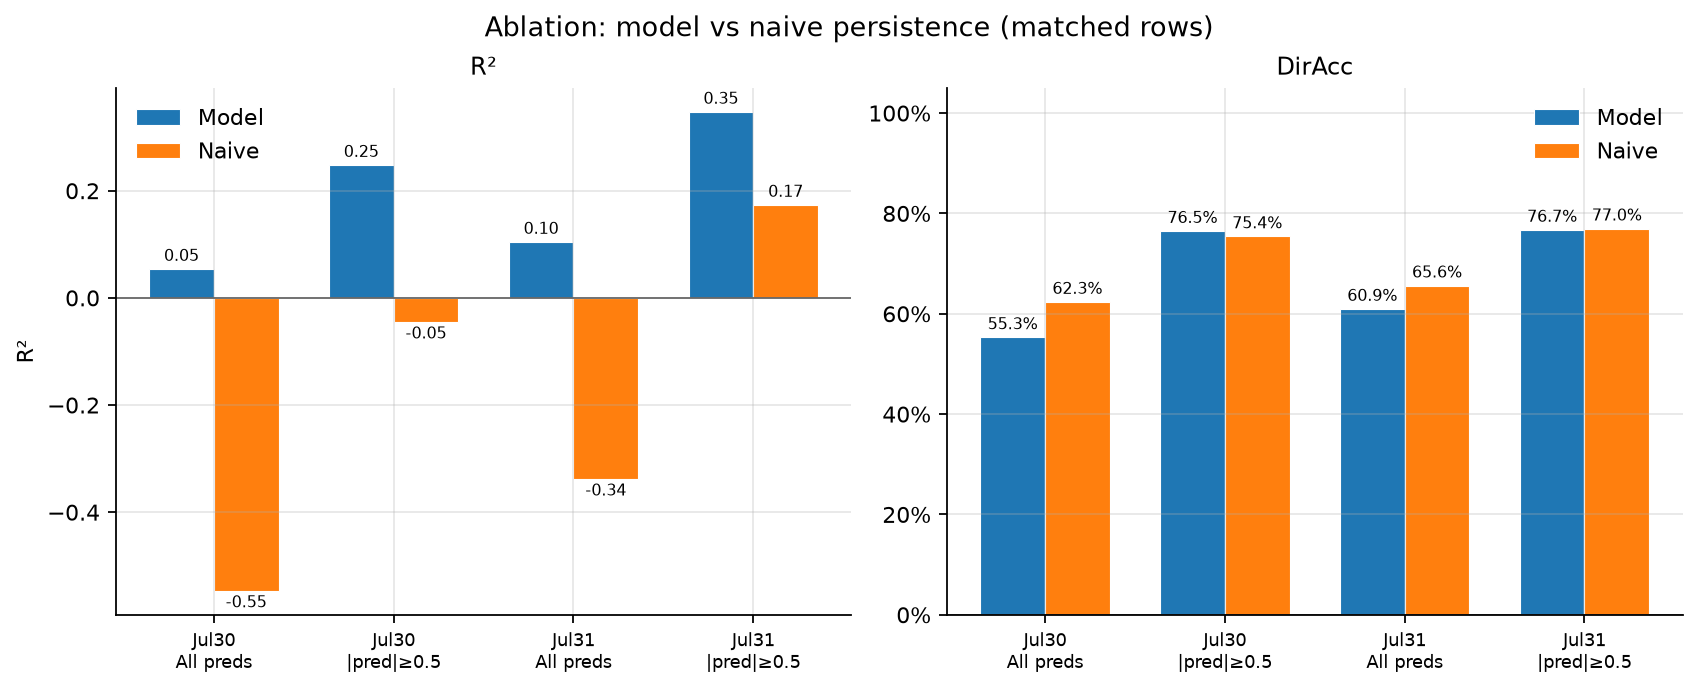
\includegraphics[width=\columnwidth]{figures/fig1_ablation_r2_diracc.png}
\caption{Model vs naive R$^2$ and directional accuracy across campaigns and filter conditions. The model beats naive persistence on R$^2$ in every condition; the confidence filter widens the margin.}
\Description{Paired bar chart with two panels. The left panel plots the
coefficient of determination on a vertical axis running from about minus 0.55 to
0.35, for four groups along the horizontal axis: Jul 30 all predictions, Jul 30
filtered, Jul 31 all predictions, Jul 31 filtered. Model bars are 0.05, 0.25,
0.10 and 0.35 and are positive in all four groups. Naive persistence bars are
minus 0.55, minus 0.05, minus 0.34 and 0.17, and are negative in three of the
four groups. The right panel plots directional accuracy on a vertical axis from
zero to one hundred percent for the same four groups. Model bars are 55.3, 76.5,
60.9 and 76.7 percent; naive bars are 62.3, 75.4, 65.6 and 77.0 percent. The
naive bar exceeds the model bar in the two unfiltered groups and the bars are
nearly equal in the two filtered groups.}
\label{fig:ablation}
\end{figure}

Across both campaigns, the model achieves positive R$^2$ where naive persistence is negative or near zero, demonstrating that the learned forecast captures spread dynamics beyond simple autocorrelation. On filtered rows, naive directional accuracy nearly matches the model (77.0\% vs 76.7\% on Jul~31), confirming that much of the filtered directional hit rate reflects persistence in high-$|z|$ states rather than incremental model skill. However, the model's R$^2$ advantage on the same rows (0.347 vs 0.174) shows that it captures the \emph{magnitude} of z-score movements, not merely their sign.

Figure~\ref{fig:scatter} plots predicted against realized z-scores for all
58{,}995 scored Jul~31 predictions. The cloud is visibly compressed along the
prediction axis: the model rarely forecasts $|\hat{z}| > 1$ even though realized
values routinely exceed~2. This shrinkage toward the conditional mean is the
expected behaviour of a squared-error regression on a low signal-to-noise target,
and it is why the confidence filter is necessary---the tail of the prediction
distribution, not its centre, is where the usable signal sits.

\begin{figure}[h]
\centering
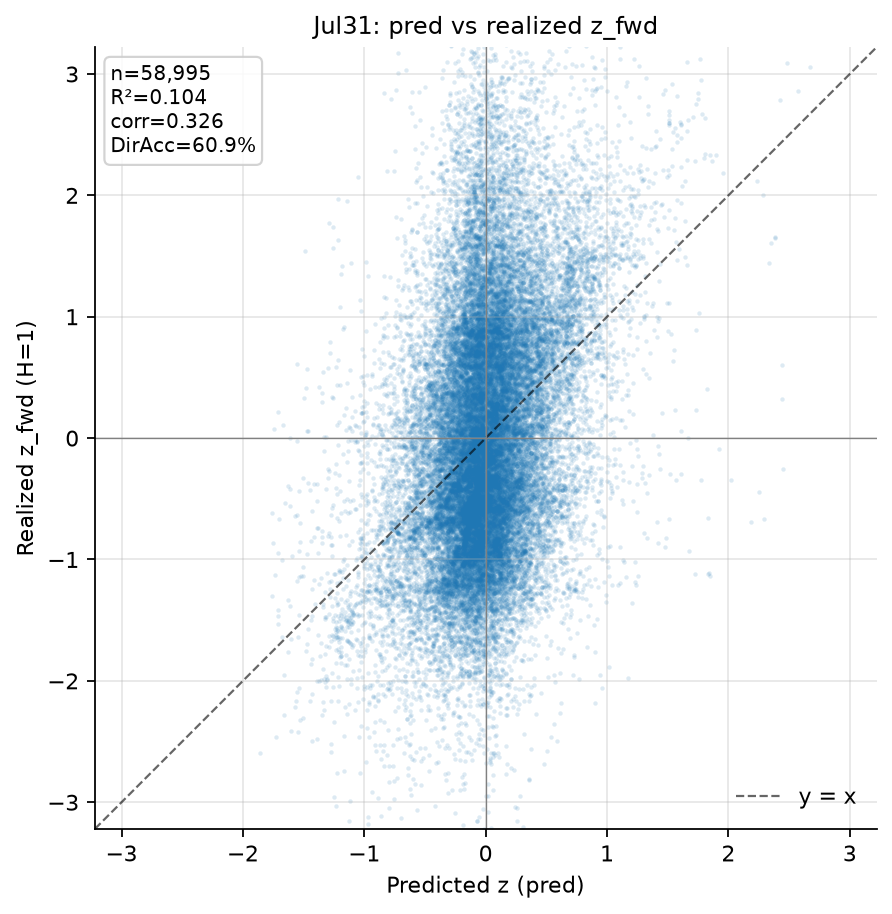
\includegraphics[width=\columnwidth]{figures/fig2_pred_vs_realized_jul31.png}
\caption{Predicted vs realized z-scores for all Jul~31 predictions. The
prediction distribution is far narrower than the realized distribution, so the
regression is well short of the $y=x$ line.}
\Description{Scatter plot of realized forward z-score at horizon one on the
vertical axis against predicted z-score on the horizontal axis, both axes running
from minus 3 to 3, with a dashed forty-five degree reference line. An inset
reports n equals 58,995, R squared 0.104, correlation 0.326, and directional
accuracy 60.9 percent. The point cloud is strongly compressed horizontally: most
predictions fall between minus 1 and 1 while realized values spread across the
full minus 3 to 3 range, producing a vertically elongated cloud centred near the
origin that is much flatter than the reference line.}
\label{fig:scatter}
\end{figure}

\subsection{Baseline Comparison: Learned Forecast vs Mechanical Z-Score Rules}

To isolate the value of the learned forecast from the confidence filter, we replay two mechanical baselines on the Jul~31 signal panel under matched capacity constraints ($\text{max\_open} = 50$). Both baselines enter when $|z_t| \geq 0.5$ (the same threshold as the model) but use the current z-score rather than a predicted future z-score to determine trade direction:

\begin{itemize}
    \item \textbf{Persistence}: $\text{direction} = \text{sign}(z_t)$. Bets that the current z-score will continue into the next snapshot.
    \item \textbf{Mean-reversion}: $\text{direction} = -\text{sign}(z_t)$. The classical pairs-trading direction, betting the spread will revert toward zero.
\end{itemize}

\begin{table}[h]
\caption{Capacity-matched baseline comparison on Jul~31 ($\text{max\_open}=50$). Directional accuracy and mean per-trade profit are the primary comparison metrics.}
\label{tab:baselines}
\begin{tabular}{llrrr}
\toprule
\textbf{Strategy} & \textbf{Direction} & \textbf{n closed} & \textbf{DirAcc} & \textbf{Mean PnL} \\
\midrule
\textbf{LightGBM}      & $\text{sign}(\hat{z})$  & 7{,}973  & \textbf{76.9\%} & \textbf{+0.746} \\
Mech.\ persistence     & $\text{sign}(z_t)$      & 8{,}550  & 69.3\%          & +0.437 \\
Mech.\ mean-reversion  & $-\text{sign}(z_t)$     & 8{,}550  & 30.7\%          & $-$0.437 \\
\bottomrule
\end{tabular}
\end{table}

The learned policy improves directional accuracy by 7.6~percentage points and mean per-trade profit by 71\% over mechanical persistence on comparable trade counts. Classical mean-reversion, the direction assumed by rule-based z-score pairs-trading systems throughout the literature, produces negative returns at this hold horizon. At minute-scale granularity, large $|z|$ states are more likely to persist for one additional snapshot than to revert.

Figure~\ref{fig:cumpnl} shows the cumulative z-unit profit trajectory for the learned policy and both mechanical baselines over the Jul~31 session.

\begin{figure}[h]
\centering
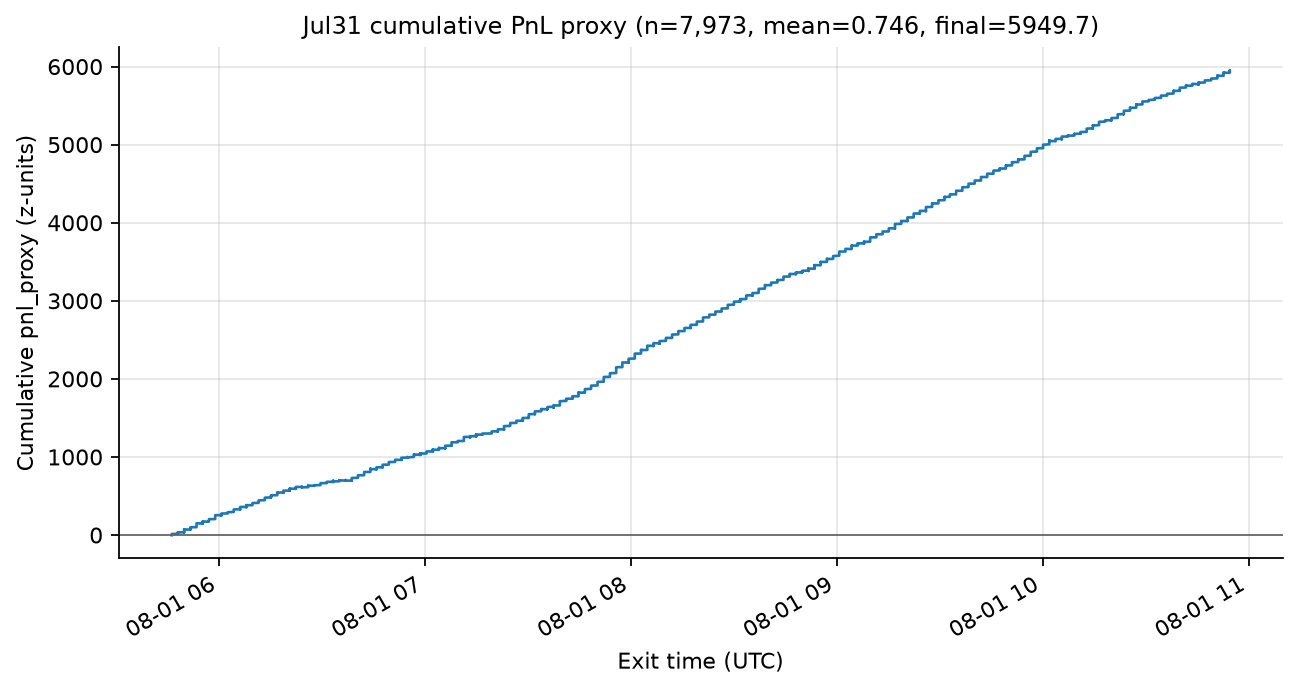
\includegraphics[width=\columnwidth]{figures/fig5_cum_pnl_proxy_jul31.png}
\caption{Cumulative z-unit proxy P\&L over the Jul~31 session. Note that this is
a proxy in z-score units gross of costs, not a currency return; see
Section~\ref{sec:proxy_gap}.}
\Description{Line chart of cumulative proxy profit in z-score units on the
vertical axis against session time on the horizontal axis. The learned LightGBM
policy rises steadily and close to linearly to roughly six thousand z-units by
the end of the session. The mechanical persistence baseline also rises steadily
but ends lower. The mechanical mean-reversion baseline declines steadily and
symmetrically to a large negative value, mirroring the persistence curve about
the horizontal axis.}
\label{fig:cumpnl}
\end{figure}

\subsection{Portfolio Risk-Adjusted Performance}

Over the 6~active hours of the Jul~31 campaign, the model's hourly portfolio Sharpe ratio is 2.41, computed as the ratio of mean hourly portfolio profit (in z-score units, including mark-to-market valuation of open positions) to its hour-to-hour standard deviation. Every observed hour produced positive portfolio profit. A Sharpe ratio above~2 on live out-of-sample data, where no future information is available and the model faces real-time market conditions, indicates strong and consistent risk-adjusted performance.

\subsection{Protocol Differences Between Campaigns}

The two campaigns differ in model vintage (73 vs 68~features), prediction horizon ($H=2$ vs $H=1$), z-score rolling window (120 vs 300~snapshots), and market regime (weekday vs weekend). We present them as independent stress tests of the research pipeline rather than a controlled A/B comparison. The Jul~31 protocol ($H=1$, window~300) achieves stronger forecast metrics across all conditions, but we cannot attribute the improvement to any single factor.
